\section{Results}

\begin{margintable}
	\vspace{-4.73cm}
	\centering
	\begin{tabularx}{1\marginparwidth}{XXd{2.2}d{2.2}d{2.2}}
		
		\toprule
		
		\textbf{Model}&\textbf{Phone}&\multicolumn{1}{c}{\textbf{0ms}}&\multicolumn{1}{c}{\textbf{33ms}}&\multicolumn{1}{c}{\textbf{66ms}} \\
		\midrule
		
		\multirow{8}{*}{\textsc{single}}   &\multirow{2}{*}{\textbf{S3}}  &12.50&13.17&14.40       \\
		&                              &(7.36)&(7.82)&(8.24)       \\
		\cmidrule(r){2-5}		
		&\multirow{2}{*}{\textbf{S4}}  &17.25&18.77&19.41       \\
		&                              &(9.94)&(10.76)&(10.78)       \\
		\cmidrule(r){2-5}						 				   
		&\multirow{2}{*}{\textbf{N5X}} &17.01&18.09&19.96       \\
		&                              &(9.76)&(10.39)&(10.93)       \\
		\cmidrule(r){2-5}										   
		&\multirow{2}{*}{\textbf{N6}}  &18.87&19.78&21.52       \\
		&                              &(11.40)&(12.15)&(12.70)       \\	
		
		\midrule
		
		\multirow{8}{*}{\textsc{general}} &\multirow{2}{*}{\textbf{S3}}   &12.95&13.48&14.52        \\
		&                               &(7.57)&(7.92)&(8.38)        \\ 
		\cmidrule(r){2-5}
		&\multirow{2}{*}{\textbf{S4}}   &16.79&17.69&18.70        \\
		&                               &(10.61)&(10.99)&(11.21)        \\
		\cmidrule(r){2-5}
		&\multirow{2}{*}{\textbf{N5X}}  &17.39&17.69&18.70        \\
		&                               &(10.61)&(10.99)&(11.21)        \\
		\cmidrule(r){2-5}									      
		&\multirow{2}{*}{\textbf{N6}}   &17.53&17.75&19.53        \\ 
		&                               &(11.59)&(11.94)&(12.72)       \\									         		
		\bottomrule    
	\end{tabularx}%
	\caption[Model results]{\small Average test euclidean distances (mm) and standard deviations (brackets) for single and general models for all configurations.}
	\label{tab:results}
\end{margintable}

\subsection{Data Set \& Preprocessing}
\label{sec:prepro}
Look at \cref{tab:baseline}
We recorded a total of 1079 minutes of sensor data from the \textit{touch} and \textit{Fitt's Law task} task. 
%Since we are only interested in sensor changes during the process of reaching for a target and touching it and the purpose of the \textit{Fitt's Law task} was only for reseting the participants grip to the lower half of the phone our first step in our preprocessing pipeline was \texttt{cutting} out the sensor fragments of the \textit{Fitt's Law task}.
Due to the high sampling rate of the sensors we first removed occurring duplicates by keeping the last sensor value and timestamp.
We then up-sampled the sensors to 333.33 Hz, resulting in 1 sample given every 3ms. 
Finally, we saved 100 samples before each touch resulting in a total of 3.456.000 samples.

Up-sampling the sensors to 1 sample every 3ms resulted in a discontinuous function for each sensor axis. 
We have therefore tried applying several smoothing procedures, including a Butterworth lowpass-filter and a moving average filter.
Both approaches, however, did not lead to an increase in accuracy, so we have adhered to the unsmoothed data of the sensors.

\subsection{Baseline}
We explored basic regressors from scikit-learn \footnote{\url{https://scikit-learn.org/stable/supervised\_learning.html\#supervised-learning}} as a baseline to test whether using novel machine learning techniques is sufficient for touch prediction with IMU.
The used regressors are abbreviated as follows: RandomForestRegressor (RF), Decision Tree Regressor (DT), K Nearest Neighbors Regressor (KNN), and Gaussian Processes Regressor (GP).
We performed a grid search for the different regressors to find the best hyperparameters for each regressor.
The results for all phones with different time configurations of all regressors can be seen in \cref{tab:baseline}.

\subsection{Neural Network Structure}
We implemented a CNN using \textit{Keras} 2.2.4 based on the TensorFlow backend. 
We trained two model types, one which we call \textit{single} and one which we call\textit{general} model.
Single models were trained on sensor and touch data of single phones; general models were trained on sensor data and normalized touch data of all phones.
The model structures differs for single and general models.
Due to place restrictions 



%\footnote{\url{https://05.jupyter.interactionlab.io/user/beneste/tree/fapra-imu}}

\begin{marginfigure}
	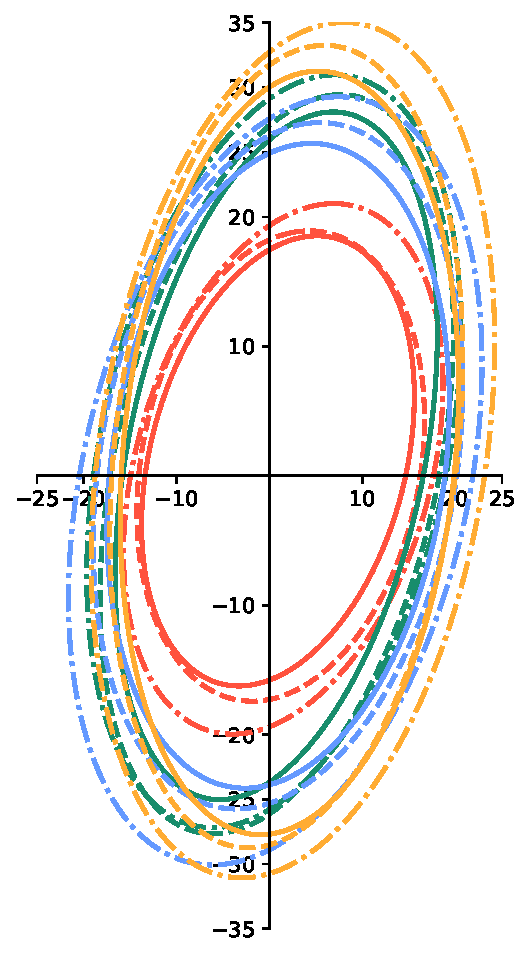
\includegraphics[height=\linewidth]{ellipses_single}
	\caption{Ellipses plot for single models.\newline}
	\label{fig:ell_single}
\end{marginfigure}

\begin{marginfigure}
	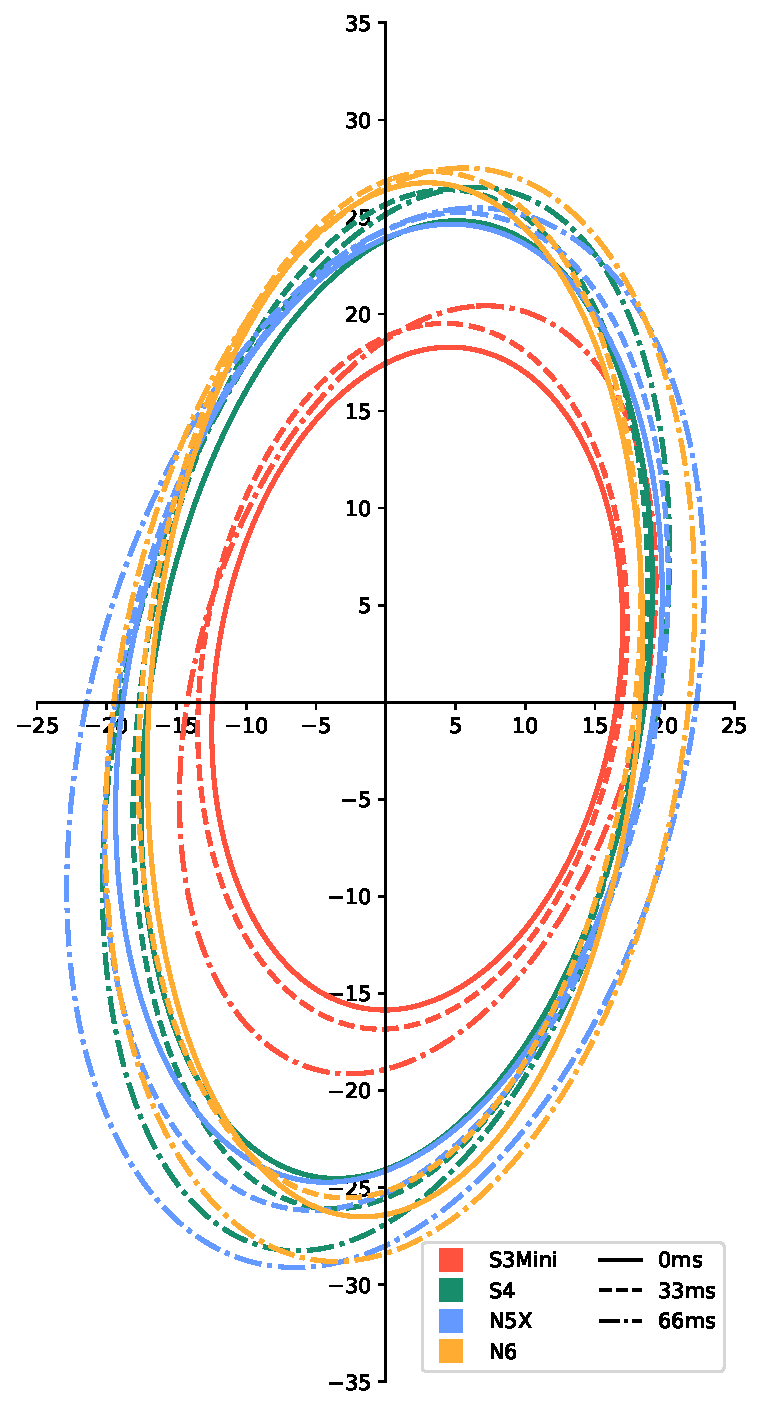
\includegraphics[height=\linewidth]{ellipses_general}
	\caption{Ellipses plot for general models.}
	\label{fig:ell_general}
\end{marginfigure}

%Report about your model. No source code!
%
%Report about the validation dataset / validation study. 